%\documentclass[a4paper,oneside,onecolumn]{article}
\documentclass[journal=nalefd,manuscript=letter]{achemso}
\usepackage{graphicx}
\usepackage{amsmath}
\usepackage{amssymb}
\usepackage{subfigure}
%\usepackage{epstopdf}
%\usepackage{setspace}
%\onehalfspace
%\usepackage{authblk}
%\usepackage[margin=2.3cm]{geometry}

%\geometry{a4paper,left=2.3cm,right=2.3cm,top=2.5cm,bottom=4.5cm}

\usepackage[version=3]{mhchem} % Formula subscripts using \ce{}
\usepackage[T1]{fontenc}       % Use modern font encodings

\newcommand{\nm}{\ensuremath{\,\textrm{nm}}}
\newcommand{\um}{\ensuremath{\,\mu\textrm{m}}}
\newcommand{\eV}{\ensuremath{\,\textrm{eV}}}
\newcommand{\uM}{\ensuremath{\,\mu\textrm{M}}}
\newcommand{\uW}{\ensuremath{\,\mu\textrm{W}}}
\newcommand{\meV}{\ensuremath{\,\textrm{meV}}}
\newcommand{\pwr}{\ensuremath{\,\textrm{kW/cm}^2}}
\newcommand{\CPS}{\ensuremath{\,\textrm{CPS}}}
\newcommand{\atto}{\ensuremath{\textrm{ATTO}\,647\textrm{N}}}

\author{Aquiles Carattino}
\affiliation[Leiden]
{Huygens-Kamerlingh Onnes, Leiden, The Netherlands}
\author{Veer Keizer}
\affiliation[Leiden]
{Huygens-Kamerlingh Onnes, Leiden, The Netherlands}
\author{Marcel Schaaf}
\affiliation[Leiden]
{Huygens-Kamerlingh Onnes, Leiden, The Netherlands}
\author{Michel Orrit}
\email{orrit@physics.leidenuniv.nl}
\affiliation[Leiden]
{Huygens-Kamerlingh Onnes Lab, 2300RA Leiden, The Netherlands}

\title{Background-free imaging of gold nanorods through detection of
anti-Stokes emission}

\keywords{Gold nanorods, Plasmon, Imaging, Anti-Stokes, Bio-imaging, Confocal}

\begin{document}
\maketitle
\abstract{This is the abstract}
\section{Introduction}
High-resolution microscopy has become an indispensable tool for studying
biological samples both in vitro and in vivo\cite{Moerner2007}.
Fluorescent organic dyes are commonly employed to such ends because of their
reduced size and high quantum yield. Fluorophores, however, have an inherent
constrain in the possible observation time, since molecules eventually bleach
under intense irradiation. Even dyes with a high photo-stability cannot be imaged for
longer than few tens of seconds. Gold nano-particles on the other hand are
almost indefinitely stable and open up many original applications including
photothermal therapy and imaging.

Gold nanoparticles do not blink nor bleach, making them ideal candidates for
labeling, tracking and manipulating biological samples over extended periods of
time. Moreover it has been shown that they don't interfere with cells'
functioning\cite{Lewinski2008}, allowing not only \em{in vitro} but also \em{in
vivo} studies. Compared to organic dyes, gold nanoparticles are much larger and
they have an emission quantum yield of the order of $10^{-6}$. This minute value
is compensated by an absorption cross section several orders of magnitude larger
than that of molecules, therefore the brightness of both particles and
fluorescent molecules is comparable.

Since the cross section of the particles scales as their volume, detecting
smaller particles in presence of background requires a different approach.
Several techniques have been proposed, including two-photon
excitation\cite{VandenBroek2013}, photothermal heterodyne
detection\cite{Berciaud2006} and interferometric detection\cite{Ignatovich2006}.
All these methods are useful but require dedicated setups and a high level of
expertise to be operated. A method that allows to image gold nanoparticles with
a high background rejection and that is readily implementable in current
confocal and wide-field microscopes would provide great benefits.

Gold nanoparticles exhibit a collective oscillation of conduction electrons
called the surface plasmon resonance. This resonance is strongly dependent on
the shape of the particles. Spheres with radius roughly between $5$ and $80\nm$
will have a resonance between $520\nm$ and $560\nm$; more elongated particles
such as nano-rods or bypiramids exhibit resonance wavelengths that reach
$800\nm$ or longer. It is important to note that tuning the shape of the particles can be
easily achieved by synthesis with a relatively narrow distribution of sizes.

The plasmon is responsible for enhanced absorption and scattering cross sections
of the particle in a specific wavelength range but it is also responsible for an
enhanced luminescence emission in the same region. The near overlap between the
excitation spectra and the emission spectra of nanoparticles makes them behave
in a different way than molecules. Upon excitation at the absorption maximum
(the plasmon resonance) most of the emission will be concentrated in a narrow
spectral region around the excitation. This implies that most of the
luminescence will be blocked by the same filters that prevent direct excitation
light from reaching the detectors.

It is also possible to excite the particles off-resonance with a
shorter wavelength laser (for instance at $532\,\nm$) and the emission will be
mostly concentrated around the plasmon resonance. This is the closest picture
to a fluorophore behavior, in which the Stokes-shifted emission can be easily
detected by introducing a long-pass filter. The drawback, however, is that the
cross section of particles is much smaller at this wavelength and can only
be compensated by increasing the excitation power. 

This work focuses in the exploitation of the anti-Sokes luminescence, which
benefits from the enhanced absorption cross section of the particles, their
photo-stability and fairly narrow emission spectra. Anti-Stokes luminescence
refers to the emission at shorter wavelengths than the excitation. When exciting
in resonance with the plasmon, a short-pass filter can be introduced for
observing only this anti-Stokes emission. The main advantage of this procedure
is that it highly reduces the background arising from self-fluorescence
and Raman-scattering from cells, opening the possiblity of imaging and tracking
smaller particles or of using lower excitation powers.

\begin{figure}[htp]
\centering
	\includegraphics[width=0.4\linewidth]{luminescence_all_AS.png}
	\caption{Schematic of the anti-Stokes luminescence arising from a single gold
	nanorod. The emission with a higher energy than the excitation energy can be
	explained by an interaction between the electron and the phonons in the metal}
	\label{fig:anti-Stokes-process}
\end{figure}

The anti-Stokes emission mechanism is depicted in Figure
\ref{fig:anti-Stokes-process} and can be described as follows: an absorbed
photon generates an electron-hole pair with an energy difference equivalent to
the energy of the incoming photon. After interacting with the gold lattice, i.e.
with a phonon, either the hole or the electron receives energy from it. This
will transiently increase the energy difference between electron and hole; if
they recombine radiatively, the emitted photon will have a shorter wavelength
(higher energy) than the incoming photon. The same mechanism can account for the
Stokes-shifted emission, where the only difference is that electron and hole
give energy to the lattice before recombining radiatively.

It has to be kept in mind that the low probability of a radiative recombination
of electron and holes implies a low quantum yield of the particles. Anti-Stokes
emission relies on electron-hole recombination after gaining energy from the
lattice and before thermalizing. Even if the anti-Stokes scenario is unlikely,
it is frequent enough as to observe an intensity in the range of $10^3$ counts
per second on an avalanche photodiode with excitation powers around $16\pwr$. We
attribute this phenomenon to an enhanced probability of emission for wavelengths
close to the plasmon resonance.

The main advantage of the approach presented in this work is the simplicity of
its implementation. Any confocal or wide-field setup that is capable of exciting
nano-particles in resonance can exploit the anti-Stokes luminescence by adding a
proper short-pass filter. Single gold nanoparticles can be detected even in
higher background conditions such as a stained cell, or a highly
self-fluorescent sample.

\section{Experimental method}

\begin{figure}[htp]
 \centering \includegraphics[width=0.45\linewidth]{Figures/01_Setup/setup_1.png}
 \caption{Experimental setup and examples of observations. a) Simplified
 schematic of the confocal microscope employed during the measurements. b) A
 typical 1-photon luminescence raster scan of the sample immersed in
 water c) luminescence spectrum of a single rod.}
 \label{fig:setup}
\end{figure}

The images of gold nanorods were recorded in a home-built confocal microscope as
sketched in Figure \ref{fig:setup}a. The objective employed was an oil-immersion
Olympus 60X NA 1.4 that allowed a high efficiency in both exciting the particles
and collecting their emission. The luminescence signal was then filtered and
detected by either an avalanche photodiode or a liquid-nitrogen-cooled
CCD-spectrometer (Acton $500\textrm{i}$). Images were acquired by scanning the
sample across the tightly focused laser beam using a XYZ piezo scanning stage
(PI Nano Cube). An example can be seen in Figure \ref{fig:setup}b. For detecting
the anti-Stokes luminescence, a $633\nm$ short-pass filter (Semrock) was added
to the detection path together with a $633\nm$ notch filter. Both filters are
needed simultaneously since either of them is not able to entirely block the
excitation light from the detectors. The Stokes luminescence was collected
replacing the short-pass filter with a long-pass.

Gold nanorods were synthesized by following standard seeded-growth
methods\cite{Nikoobakht2003}. The average size of the nanorods was $50\nm\times
20\nm$ and their SPR is located at around $630\nm$ in water (refer to the
Supplementary Information for SEM images and bulk extinction spectra of nanorods
as synthesized). Samples were prepared by spin casting a suspension of gold
nanorods onto a clean coverslip. 

Lasers with two different wavelengths were employed. A $532\nm$ laser (CNI) was
used for exciting the transverse plasmon and collect the full longitudinal
plasmon spectrum. Single nanorods exhibit a narrow Lorentzian shape as
displayed in Figure \ref{fig:setup}c, and therefore this characterization is
useful for discarding clusters of particles from the analysis. A second laser
(Thorlabs HeNe) with a wavelength of $633\nm$ allowed us to excite the particles
in resonance and collect either the Stokes or the anti-Stokes emission depending
on the introduced filters.

\begin{figure}[htp]
\centering
	\subfigure{%
	\includegraphics[width=0.4\linewidth]{intensity_vs_plasmon_LP.png}}
	\subfigure{%
	\includegraphics[width=0.4\linewidth]{intensity_vs_plasmon_SP.png}}
	\caption{Emission intensity as a function of plasmon peak position for the
	Stokes (a) and anti-Stokes (b) sides. The spread in intensities for similar
	peak position can be attributed to variations in sizes or different
	orientations of the rods in a non perfectly circularly polarized beam.}
	\label{fig:emission_peak_position}
\end{figure}

Figure \ref{fig:emission_peak_position} shows the dependence of the emission
intensity as a function of the plasmon peak position for the Stokes and the
anti-Stokes components. The inhomogeneity observed can be attributed to a
distribution of sizes of the rods (bigger particles will have a bigger cross
section). It is possible to observe that the maximum emission intensity for the
anti-Stokes appears for those particles with their plasmon slightly blue-shifted
from the laser wavelength, while the opposite is observed for the Stokes
emission. This means that there is a trade-off between the excitation efficiency
and the collection efficiency: exciting in perfect resonance is more efficient,
but the filters will eliminate most of the luminescence. Therefore, exciting
slightly to the blue (red) of the resonance will be beneficial for the
(anti-)Stokes imaging.

For proving that the technique is well suited for imaging of particles in
biological conditions, HeLa cells were deposited on top of the nanorod samples.
This procedure ensures that the analysis is performed on single-particles and
therefore any intensity comparison is not arising from clusters of nanorods.
It also allowed us to characterize their emission both by acquiring spectra or
by studying the dependency with excitation power, avoiding their diffusion out
of focus. It may be argued that this scenario is not exactly imaging of rods in
cells, but resembles very well imaging in cell membranes without going into the
details of the functionalization of the particles.

\begin{figure}[htp]
\centering
	\includegraphics[width=0.4\linewidth]{Figures/02_White_Light/White_Light_with_phone.jpg}
	\caption{White light transmission image of the sample with cells deposited on
	top of the rods. It is possible to observe that they cover entirely the
	observed region without spacing in between them. The spherical cells seen out
	of focus are cells that can't attach to the glass, remaining with that shape.}
	\label{fig:white-light}
\end{figure}

We have also acquired images of nanoparticles under stained cells. This was
achieved by incubating the cells already attached to the coverslips with $\atto$
for approximately half an hour. This set of experiments allowed us to compare
Stokes and anti-Stokes emission in a high-background condition. Figure
\ref{fig:white-light} shows a typical white light transmission image of the
samples. The high confluency allows to confirm that cells cover uniformly the
entire observed area. In this way we can assure that the studied nanorods are
always below a cell.


\section{Results and discussion}

\begin{figure}[htp]
\centering
	\includegraphics[width=0.4\linewidth]{3_Curves.png}
	\caption{Luminescence spectra of a single gold nanorod excited with a $532\nm$
	laser (green curve). The Stokes emission after excitation with a $633\nm$
	HeNe laser is the red curve and the blue curve corresponds to the anti-Stokes
	emission. These last two curves were normalized such that the Stokes emission
	overlaps the spectrum obtained with the $532\nm$ laser.}
	\label{fig:spectra_rod}
\end{figure}

Figure \ref{fig:spectra_rod} shows typical spectra of a gold nanorod under
different excitation wavelengths. The green curve is the one-photon-excited
luminescence spectrum observed while irradiating with the $532\nm$ laser; the
full spectrum of the longitudinal plasmon is clearly observable with its
resonance at $620\nm$. If the particle is excited at or close to this resonance,
the shape of the spectrum changes drastically: the red curve shows the Stokes
shifted emission while exciting at $633\nm$. To show the overlap with the
curve obtained with the $532\nm$ laser, the Stokes curve was divided by a
constant such that both have the same value at $650\nm$, just above the cutting
wavelength of the long-pass filter. The blue curve displays the anti-Stokes
emission at shorter wavelengths with the same normalization constant used for
the Stokes case. The spectral shape of this emission doesn't resemble that of
the plasmon resonance as was the case for the longer wavelengths.

The dashed curves in the Figure correspond to the anti-Stokes and Stokes
emissions without normalization. For this nanoparticle, the count rate for both
types of emissions is comparable, and they are also comparable to the
luminescence intensity obtained while exciting at $532\,\nm$. The main
difference is the laser intensity employed; the power density for exciting the
transverse plasmon with the $532\nm$ laser was set to $80\pwr$, while for both
the anti-Stokes and Stokes, the $633\nm$ laser was set to $16\pwr$, $5$ times
less intense. 

\begin{figure}[htp]
\centering
	\subfigure{%
	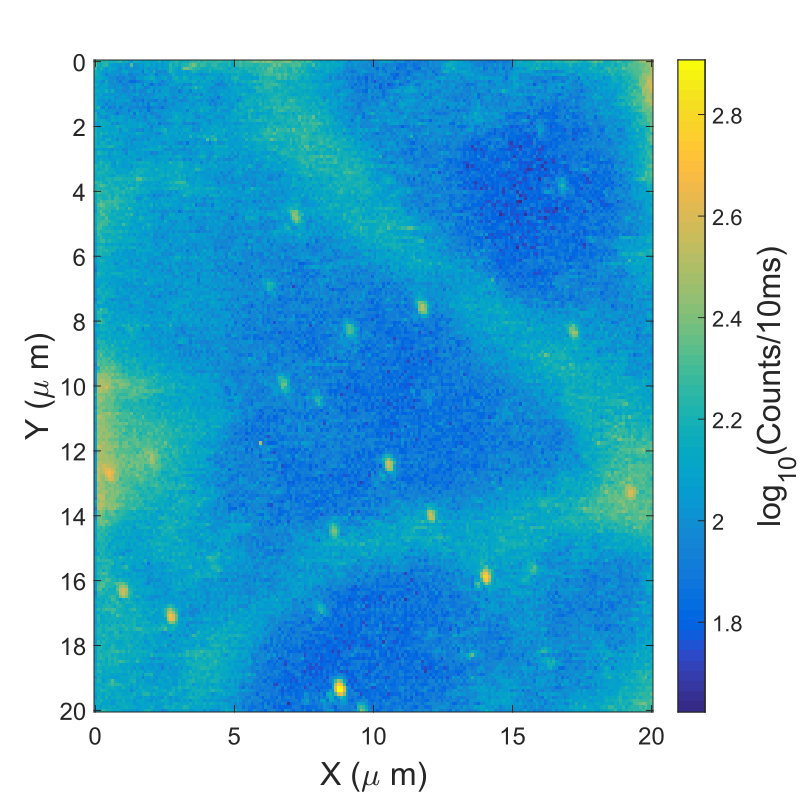
\includegraphics[width=0.4\linewidth]{Figures/03_Stokes_AS/scan05.png}}
	\subfigure{%
	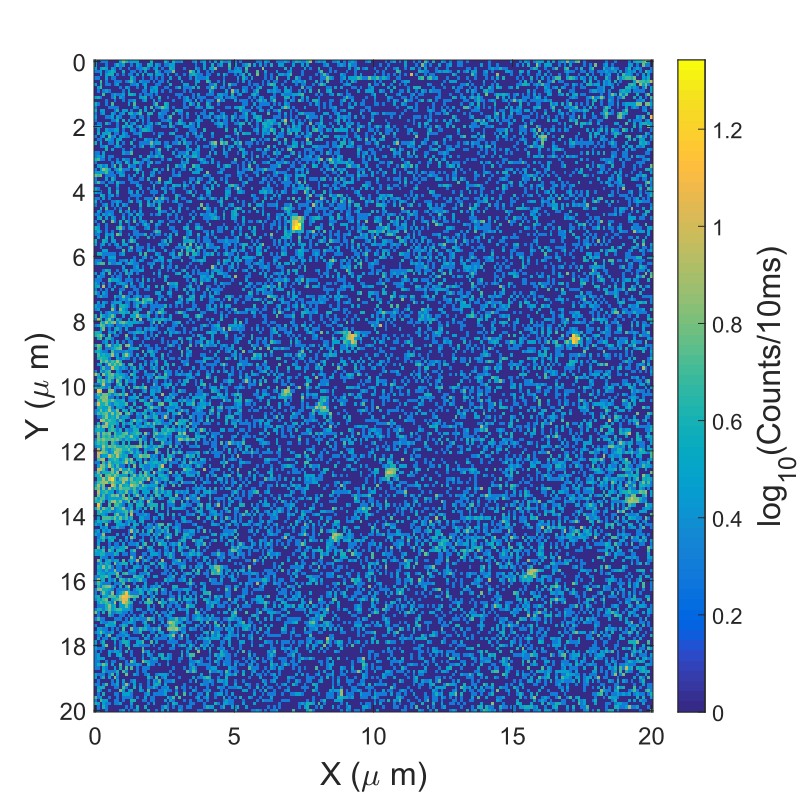
\includegraphics[width=0.4\linewidth]{Figures/03_Stokes_AS/scan06.png}}
	\caption{Raster scan using a long pass filter (a) and a short pass filter (b).
	The same rods can be observed; it has to be noted that not necessarily the
	brightest in the Stokes emission will be the brightest in the anti-Stokes.}
	\label{fig:shortpass_longpass}
\end{figure}

Figure \ref{fig:shortpass_longpass} shows two raster scans of the same
$15\times15\um^2$ area of the sample with HeLa cells on top of gold
nanorods. The left image shows the Stokes emission, where a $633\nm$ notch and
$633\nm$ long pass filter were employed. The right image corresponds to the
anti-Stokes emission, where the same notch and a $633\nm$ short pass filter were
employed. In both cases the irradiation intensity was kept at $120\uW$ at
the back aperture of the objective. The same particles are observed with both sets
of filters but the main difference between the two is the background count rate.
In the Stokes image a highly structured background can be observed; we
attribute this emission to self-fluorescence of the cell. The anti-Stokes
image shows a much lower and flatter background and highly distinguishable
single particles. Both images display the absolute count rate obtained without any
further dark count subtraction. 

\begin{figure}[htp]
\centering
	\subfigure{%
	\includegraphics[width=0.4\linewidth]{Figures/03_Stokes_AS/hist_scan05_log.png}}
	\subfigure{%
	\includegraphics[width=0.4\linewidth]{Figures/03_Stokes_AS/hist_scan06_log.png}}
	\caption{Pixel intensity distribution for anti-Stokes and Stokes emission.}
	\label{fig:distribution_pixels}
\end{figure}

Figure \ref{fig:distribution_pixels} shows the distribution of pixel intensities
in both images. The Stokes image shows a distribution of values centered around
$5500$ counts per second (CPS), while the anti-Stokes shows the vast majority of
the pixels with less than $100\CPS$, roughly coinciding with the dark counts of
the detector. This already is a big indication that most of the background in
the anti-Stokes case arises from the detector and not from the sample. This is
however not true in the entire image. The region close to the origin,
coordinates ($0,0$) shows a slightly higher emission in both cases. This may be
due to anti-Stokes Raman emission from the cell itself which cannot be
blocked with a short pass filter.

To prove the usefulness of the method in situations with higher
backgrounds, we incubated the cells with a solution of \atto.
The staining of the cell, even if not specific, results in a similar situation
to what would be obtained in the case of labeling of particular organelles or
the entire cell membrane. This dye was chosen because its absorption maximum is
close to $633\nm$, the excitation wavelength we employed in these
experiments, but also because of its photo stability and high quantum yield.

\begin{figure}[htp]
\centering
	\subfigure{%
	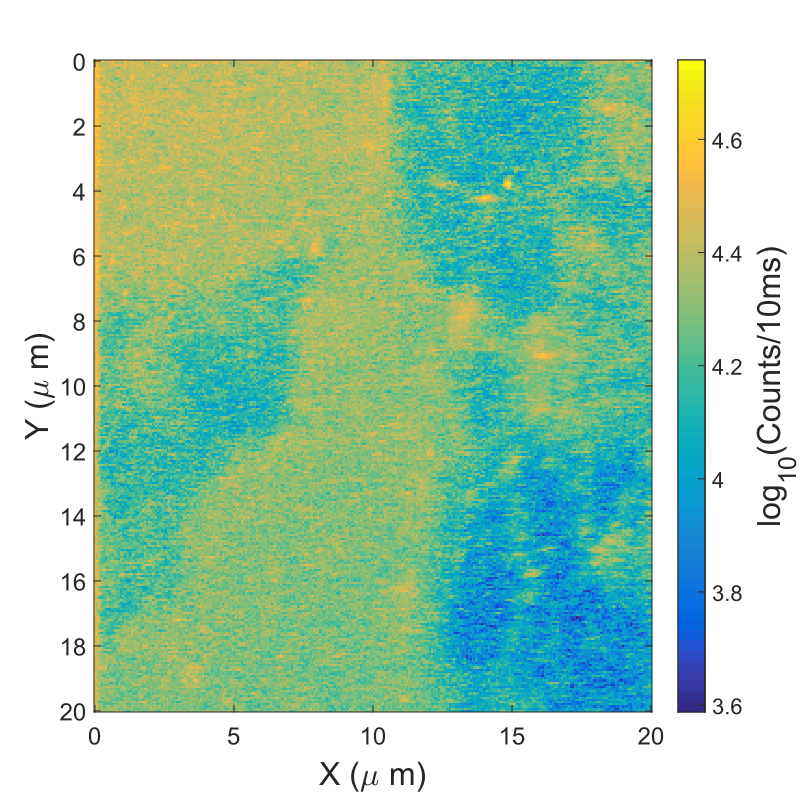
\includegraphics[width=0.4\linewidth]{Figures/04_Stokes_AS_with_dye/scan03.png}}
	\subfigure{%
	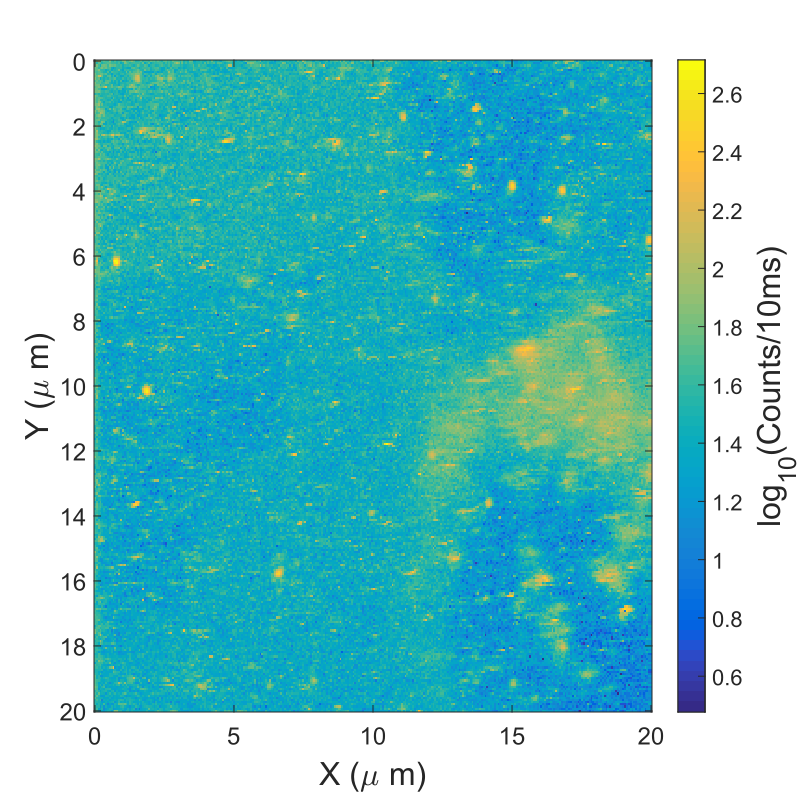
\includegraphics[width=0.4\linewidth]{Figures/04_Stokes_AS_with_dye/scan04.png}}
	\caption{Raster scan using a long pass filter (a) and a short pass filter (b).
	The same rods can be observed; it has to be noted that not necessarily the
	brightest in the Stokes emission will be the brightest in the anti-Stokes.}
	\label{fig:Stokes_AS_with_dye}
\end{figure}

Figure \ref{fig:Stokes_AS_with_dye} shows two raster scans of the samples
described above. The left shows the anti-Stokes result, in which
single-particles are clearly distinguishable. The right one shows the Stokes
emission, in which at most one particle can be clearly distinguished from the
background and is marked with a circle. The distribution of intensities in
Figure \ref{fig:hists_dye} show a clear change as compared to the situation without
dye. The anti-Stokes maximum is closer to $500\CPS$, higher than
the dark counts of the detector. The Stokes emission, on the other hand shows a
distribution centered around $200\textrm{kCPS}$, one order of
magnitude higher than the observed without the dye.

\begin{figure}[htp]
\centering
	\subfigure{%
	\includegraphics[width=0.4\linewidth]{Figures/04_Stokes_AS_with_dye/hist_scan03.png}}
	\subfigure{%
	\includegraphics[width=0.4\linewidth]{Figures/04_Stokes_AS_with_dye/hist_scan04.png}}
	\caption{Pixel intensity distribution for anti-Stokes and Stokes emission.
	The cells were stained with \atto.}
	\label{fig:distribution_pixels}
\end{figure}

These results indicate that the Stokes imaging deteriorates much faster than the
anti-Stokes in the presence of emitting molecules both from the cell itself or
from the dye added \textit{a posteriori}. The images show regions with higher
emission intensities in both configurations, most probably due to a higher concentration
of dye in particular regions of the cell. At much higher concentrations than
the ones employed in this work, the dye has also shown anti-Stokes emission at
rates even higher than the particles, meaning that a balance has to be obtained
to still be able to detect the particles.

\begin{figure}[htp]
\centering
	\subfigure{%
	\includegraphics[width=0.4\linewidth]{Figures/03_Stokes_AS/pcle3.png}}
	\subfigure{%
	\includegraphics[width=0.4\linewidth]{Figures/04_Stokes_AS_with_dye/pcle3.png}}
	\caption{Emission intensity as a function of excitation intensity for: the
	Stokes emission (of both the particle and the background) and the anti-Stokes
	emission. A particle with the plasmon close to the laser line was chosen as to
	avoid favouring one or the other emission.}
	\label{fig:power_intensity}
\end{figure}

Figure \ref{fig:power_intensity}a shows the dependence of the acquired
luminescence and the background as functions of excitation power for both the
Stokes and anti-Stokes emissions of a particle bellow a cell without dye. Care
was taken in choosing a particle with a resonance close to the laser resonance,
not to favor nor the Stokes nor the anti-Stokes luminescence. The Stokes
emission (red curves) shows a linear increase in signal together with a linear
increase in background. In this case the signal-to-background ratio saturates at
a value of $5$. The anti-Stokes emission (blue curves) however shows a much
steeper increase of the signal than the background, reaching a
signal-to-background ratio of $10$. The signal-to-background ratio of the
anti-Stokes is two-fold higher than the Stokes one. Particles with a plasmon
resonance to the blue of the laser wavelength show an even higher difference
between both types of emission.

Figure \ref{fig:power_intensity}b shows the same type of curves than
\ref{fig:power_intensity}a, but for a particle under cells that were stained
with \atto. It can readily be seen that in the Stokes case the particle is
barely above the signal arising from the background, and the
signal-to-background ratio in the order of $3$. On the other hand, the
anti-Stokes luminescence shows an enhanced contrast, reaching a
signal-to-background ratio of more than $11$. This particle was chosen because
it was one of the few observable with the long-pass filter; most of the
particles that were observable with the anti-Stokes luminescence didn't display
an emission brighter than the background in the Stokes configuration, as shown
in Figure \ref{fig:Stokes_AS_with_dye}.

When the cells were stained with \atto, we observed an increase in the
background level for both Stokes and anti-Stokes emission and they also depend
on excitation power. The Stokes emission is expected to be linear with
irradiation power, since it is the result of fluorescence from the dye and can
be seen in fig \ref{fig:power_intensity}b. On the other hand, the increase in
the anti-Stokes background can be attributed to anti-Stokes emission from the
dye itself; it is of no surprise that a molecule absorbing laser light exhibits
this emission at room temperature. The main difference between both curves is
the slope at which the background increases. The Stokes emission of the
background raises as steeply as the particle's emission with increasing
excitation power; the anti-Stokes background however, shows a much more gradual
increase than the particle's emission.

The signal-to-background ratio of the anti-Stokes emission increases with
increasing laser excitation powers, going from values close to $2$ for $10\uW$
up to values of $11$ for $150\uW$ as shown in fig \ref{fig:power_intensity}b.
However this can't be extrapolated further than the results here presented. It
is known that gold nano rods reshape under high irradiation intensities. For
high-NA objectives like the one employed in this work, a rule of thumb is not to
exceed $150\uW$ at the back aperture to prevent reshaping.

\section{Conclusions}
In this work we have proved that anti-Sokes emission arising from the excitation
in (or close to) the plasmon resonance of a gold nanorod can be exploited to
image them in biologically relevant conditions. The comparison between the
Stokes and anti-Stokes was possible by using particles immobilized on the
substrate, but this work shows that the technique can be easily extended to
imaging in fixed cells, in vivo or even for tracking particles in real time.

Extending this technique to wide-field should be possible considering the laser
powers employed in this work. EMCCDs provide enough gain as to easily detect
single nanoparticles, while at the same time the background is sufficiently low
as to give a high contrast. This extension of the technique would provide a way
of doing tracking at higher framerates than achievable by confocal imaging.

The lower count rate of the anti-Stokes compared to the Stokes emission can be a
drawback in some applications as localization. This technique's accuracy depends 
on the number of photons detected, and is given by $\approx
1/\sqrt{N}$, where $N$ is the number of photons collected. The count rates
obtained in this work are close to $1.5\,\textrm{kCPS}$, and should be enough
for many applications. 

We have shown that the signal-to-background ratio of the anti-Stokes emission is
higher than for the Stokes emission. In the case of non stained HeLa cells,
typical values can be around $10$ and $5$ respectively for a particle with a
resonance equal to the laser wavelength. For stained cells the difference is
much more remarkable, since most of the particles will have a Stokes emission
comparable to the background, while in the anti-Stokes the signal-to-background
ratio can still be higher than $10$.

The main advantage of the technique presented in this work is that it can be
easily implemented in any commercial or home built microscope. It does not
require a high investment nor in equipment nor in time, since filters are
normally available for common laser wavelengths and there is no further need of
modifying any experimental configuration already existent. Moreover all the data
analysis techniques employed in confocal or wide-field images for localization,
tracking, etc. do not need to be modified. 


\bibliography{BackgroundFree}{}

\end{document}
